\documentclass[slovak, master]{diploma}

% Packages (balíky makier)
\usepackage[autostyle=true, czech=quotes]{csquotes} % korektná sadzba úvozoviek, podpora pre balík biblatex
\usepackage[backend=biber, style=iso-numeric, alldates=iso]{biblatex} % bibliografia
\usepackage{dcolumn} % stĺpce tabuľky s číselnými hodnotami
\usepackage{subfig} % makrá pre "podobrázky" a "podtabuľky"
\usepackage[csharp]{diplomalst} % sádzanie
%\usepackage[python]{diplomalst}
%\usepackage{tcolorbox} % oramovanie

% ------------------------------------------------------

% Definované vlastné metódy, triedy a príslušné farby
% viz bakalarka

% ------------------------------------------------------

% Nový druh tabuľkového stĺpca, v ktorom sú čísla zarovnané podľa desetinnej čiarky
%\newcolumntype{d}[1]{D{,}{,}{#1}}

% Odstranenie warningov s underfull vbox
%\raggedbottom

% Nastavenie tex color boxu
%\newtcbox{\mybox}[2][black]{outer arc=0pt,  boxsep=0pt, left=0pt, right=0pt, top=0pt, bottom=0pt, boxrule=2pt}

% ------------------------------------------------------

%Zásady pro vypracování
% S umělou inteligencí, která je zodpovědná za rozhodování, se setkáme ve většině počítačových her, ať už jde o hry deskové, plošinové nebo např. tahové. Cílem této diplomové práce je naimplementovat herní prostředí, v němž budou pro rozhodování použity klasické algoritmy jako např. ID3, C4.5, CART (regresní stromy), CHAID (Chi-square, automatic interaction detection), MARS ( (multivariate adaptive regression splines), náhodný les (random forest) a algoritmy jako Deep Q-learning, Double Deep Q-learning, popř. hluboké neuronové sítě a tyto metody porovnat na základě experimentů a následné statistické analýzy. Metody budou porovnány na základě výkonu a úspěšnosti z hlediska řešení daných problémů.

% Zásady pro vypracování:
% 1. Seznamte se s algoritmy jmenovanými výše a způsobem jejich použití v počítačových hrách.
% 2. Navrhněte vlastní netriviální počítačovou hru, kde budou vybrané algoritmy použity pro rozhodování tzv. NPC (non-playing character). Při výběru algoritmů je potřeba, aby byly zastoupeny obě kategorie výše zmíněných algoritmů - tzn. klasické i algoritmy strojového učení. Celkem by mělo být použito aspoň 5 algoritmů, kde aspoň 2 budou patřit do kategorie strojového učení. Ve hře bude implementována postava hráče, který bude proti NPC bojovat.
% 3. Naimplementujte zvolené algoritmy a proveďte jejich srovnání na základě opakovaných experimentů. Během implementace klaďte důraz na efektivitu. Žádný z algoritmů nesmí být proti jinému zvýhodněn. Proveďte statistickou analýzu a s použitím vhodných statistických testů vyhodnoťte kvalitu poskytovaného řešení těchto algoritmů a jejich výkon.
% 4. Výsledky zpracujte v podobě tabulek a grafů a na jejich základě proveďte vyhodnocení testů. Shrňte výhody a nevýhody jednotlivých algoritmů. V závěru uveďte, který algoritmus dosáhl nejlepšího výkonu a který byl při řešení daných úkolů nejúspěšnější.

% ------------------------------------------------------

% Titulná strana
\ThesisAuthor{Bc. Miroslav Kačeriak}
\ThesisSupervisor{prof. Ing. Jan Platoš, Ph.D.}
\CzechThesisTitle{Rozhodování v počítačových hrách - srovnání metod umělé inteligence}
\EnglishThesisTitle{Decision Making in Computer Games - a Comparison of Artificial Intelligence Methods}
\ThesisAssignmentFileName{ThesisSpecification_KAC0067_vsboee22026009.pdf}
\SubmissionYear{2023}

% ------------------------------------------------------

% Abstrakty
\CzechAbstract{TODO}

\CzechKeywords{spätnoväzobné učenie, rozhodovacie stromy, ID3, D4.5, CART, Unity engine, C\#, Python}

\EnglishAbstract{TODO}

\EnglishKeywords{reinforcement learning, decision trees, ID3, D4.5, CART, Unity engine, C\#, Python}

% ------------------------------------------------------

% Poďakovanie
\Acknowledgement{Rád by som na tomto mieste poďakoval prof. Ing. Jánovi Platošovi, Ph.D. za pomoc a ochotu prejavenú popri vedení tejto diplomovej práce a mojej priateľke Zdenke za trpezlivosť a prínosné rady, bez ktorých by výsledná práca bola o niečo chudšia.}

% ------------------------------------------------------

% Skratky
\AddAcronym{NPC}{Non-Playable Character}
\AddAcronym{CART}{Classification and Regression Tree}

% ------------------------------------------------------

% Literatúra
%\addbibresource{literature.bib}

% ------------------------------------------------------

% Samotný dokument
\begin{document}
\MakeTitlePages

% Zoznam obrázkov
\listoffigures
\clearpage

% Zoznam tabuliek
\listoftables
\clearpage

% Zoznam zdrojakov
\lstlistoflistings
\clearpage

% Chapter 1
\chapter{Úvod}
\label{sec:Introduction}
%TODO

% ------------------------------------------------------

% Teória
% Chapter 2
\chapter{Umelá inteligencia v hrách}
\label{sec:AI in games}
%TODO

\section{Rozhodovacie stromy}
\label{sec:DecisionTreesOverview}

\section{Strojové učenie}
\label{sec:MachineLearningOverview}
%TOOD
\subsection{Spätnoväzobné učenie}
\label{sec:ReinforcemenLearningOverview}
%TODO

% ------------------------------------------------------

% Vypracovanie
% Chapter 3
\chapter{Použité technológie}
\label{sec:Tech}
%TODO
\section{Unity Engine}
\label{sec:Unity}
%TODO
\section{Nástroj ML-Agents}
\label{sec:ML-Agents}
%TODO
%...?

% Chapter 4
\chapter{Hra a herné prostredie}
\label{sec:GameOverview}
Táto kapitola je venovaná vytvorenej hre a všetkým jej aspektom, či princípom fungovania. Prvá sekcia tejto kapitoly si kladie za cieľ popísať žánrové aj príbehové zasadenie hry. V ďalších sekciách je potom podrobne prebraté fungovanie jednotlivých aspektov a herných mechaník, s dôrazom na zmyslové vnímanie jednotlivých NPC agentov.

\section{Žáner a príbehové zasadenie}
\label{sec:GenreAndSetting}
Hra samotná má svojou hrateľnosťou najbližšie k žánru stealth. Tento žáner sa vyznačuje tým, že hráč sa snaží vyhnúť odhaleniu a následnému priamemu stretu s nepriateľom. K dosiahnutiu cieľa je teda využívaný pomalý a tichý postup, kde každý krok by mal byť dobre premyslený a načasovaný. 

Príbeh hry je zasadený do pirátskeho prostredia. Hráč sa ocitá v roli radového člena pirátskej posádky, ktorá bola napadnutá flotilou anglického námorníctva. S vypätím všetkých síl sa mu na poškodenom záchrannom člne podarilo dostať na najbližší obývaný ostrov, kde však zisťuje, že nie je všetko v poriadku. Namiesto obyvateľov ostrova nachádza len agresívnych kostlivcov. 

Hráčovou úlohou je nájsť na ostrove funkčný čln, pozbierať zásoby nutné na ďalšiu plavbu a pokiaľ možno pri tom nevzbudiť pozornosť.

\begin{figure}[!htbp]
	\centering
	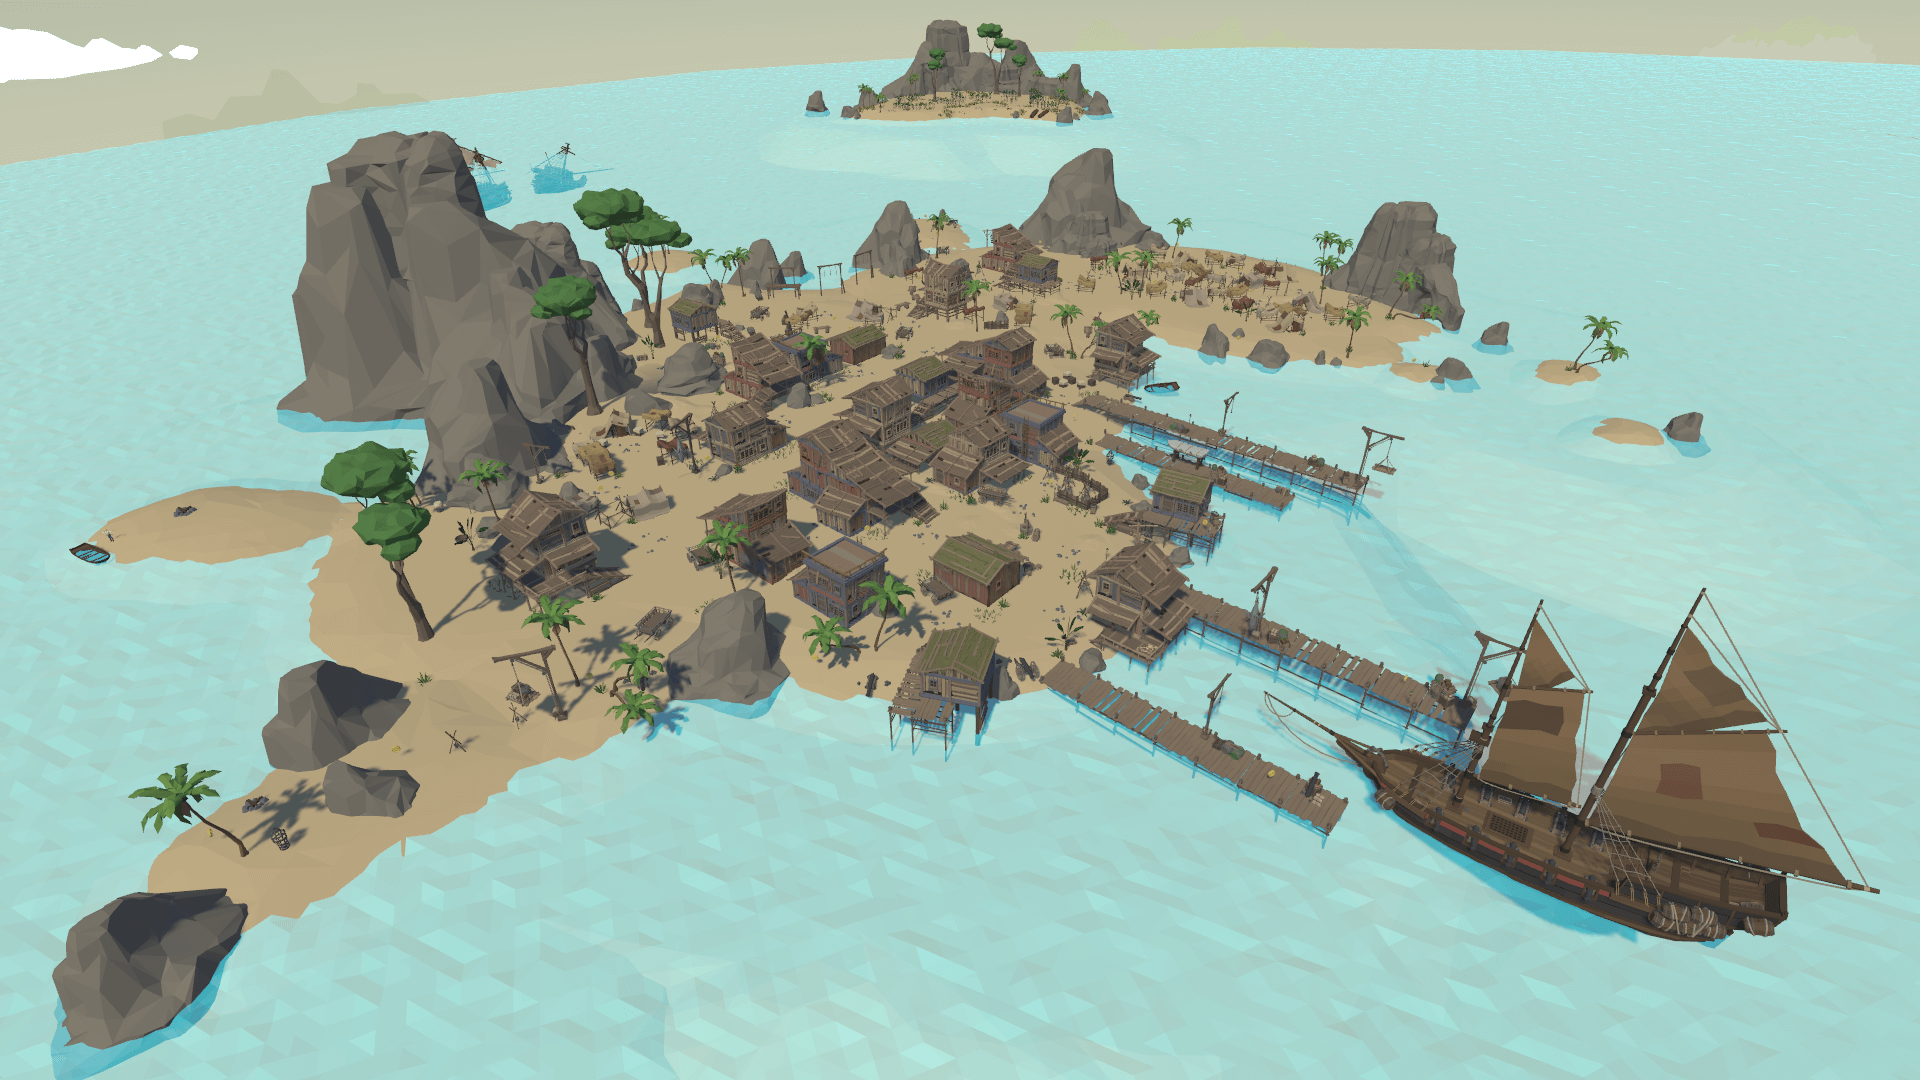
\includegraphics[width=.9\textwidth]{Figures/game_compressed.png}
	\caption{Vyrenderovaná snímka z hry}
	\label{pic:GameScreenshot}
\end{figure}

\section{Štruktúra hry}
\label{sec:GameStructure}
%TODO
%spomenut synty tu
%manazeri overview
Hra je rozdelená do dvoch samostatných scén. Konkrétne ide o hlavnú scénu, kde sa odohráva samotná herná slučka a scénu s hlavnou ponukou. V editore Unity je možné medzi jednotlivými scénami ľubovoľne prepínať, prípadne mať aktívnych niekoľko scén naraz. V samostatnom zostavení aplikácie je však nutné vybrať, ktoré konkrétne scény budú prítomné. Každá scéna potom dostane poradové číslo, tzv. build index a scéna s číslom nula, v tomto prípade hlavná ponuka, bude spustená ako prvá. Scéna s hlavnou ponukou je bližšie popísaná v sekcií \ref{sec:MainMenuAndUI}.

Scénu je potom možné chápať ako koreňový adresár pre hierarchiu herných objektov. Jednotlivé herné objekty je teda možné vložiť do scény samostatne alebo ako potomka iného herného objektu. Manipulácia s pozíciou, rotáciou či mierkou rodiča sa teda aplikuje aj na potomka. Naopak to však neplatí. Z tohto dôvodu sa rozlišujú dve súradnicové sústavy, a síce globálna (celková) a lokálna (relatívna voči predkovi). Využitie globálnej súradnicovej sústavy však vyžaduje vziať do úvahy parametre všetkých predkov daného objektu v scéne, čo nie je ideálne z hľadiska výkonu. Preto bol v projekte preferovaný lokálny súradnicový systém napríklad na herných NPC agentov či predmety, ktoré je v hre možné zbierať a je pre nás zaujímavá ich pozícia. Predkovia týchto objektov sú potom umiestnení v počiatku súradnicovej sústavy, čo zaisťuje konzistenciu.

V každej scéne sa nachádza objekt MainManager, ktorý slúži ako prístupový bod k ostatným manažérom. Typicky ide o objekty ConfigManager, GameManager, InputManager a SoundManager, nie všetky sú však nutné v každej scéne. 

Krátky popis jednotlivých manažérov:
\begin{itemize}
  \item \textbf{Objekt ConfigManager} -- je prístupovým bodom k nastaveniam hry, zaisťuje serializáciu a deserializáciu dát, rovnako ako ich perzistentnosť po každej zmene.
  \item \textbf{Objekt GameManager} -- reštartuje scénu pri smrti alebo výhre hráča, kontroluje prerekvizity výhry, aktualizuje grafické užívateľské rozhranie pri získaní predmetu a zobrazuje kontextovú ponuku na ukončenie hry či návrat do hlavnej ponuky po stlačení príslušnej klávesy.
  \item \textbf{Objekt InputManager} -- je abstrakciou nad konkrétnou implementáciou získavania hráčskeho vstupu, čo umožňuje na jednom centrálnom mieste zmeniť tzv. starý input systém za nový, či naopak, prípadne z testovacích dôvodov hráčsky vstup úplne ignorovať. 
  \item \textbf{Objekt SoundManager} -- Vyvoláva simuláciu zvuku, na ktorý môžu zareagovať NPC agenti v dosahu.
\end{itemize}

\subsection{Herná slučka}
\label{sec:GameLoop}
%TODO
\subsection{Hlavná ponuka a užívateľské rozhranie}
\label{sec:MainMenuAndUI}
%TODO
%TODO
\subsection{Perzistentné nastavenia hry}
\label{sec:Settings}
%TODO
%\subsection{Ovládanie hry} % Nie je to skor do hraca?
%\label{sec:Input}
%TODO

%TODO

\section{Štruktúra hráčskej postavy}
\label{sec:Player}
%TODO
\subsection{Ovládanie hry}
\label{sec:Input}
%TODO
\section{Štruktúra NPC agentov}
\label{sec:Agents}
%TODO
%NAVMESH
\subsection{Zmyslové vnímanie agentov}
\label{sec:Perception}
%TODO

% Chapter 5
\chapter{Rozhodovanie agentov s využitím rozhodovacích stromov}
\label{sec:ImplDecisionTrees}
%TODO
\section{Algoritmus ID3}
\label{sec:ID3}
%TODO
\section{Algoritmus D4.5}
\label{sec:D45}
%TODO
\section{Algoritmus CART}
\label{sec:CART}
%TODO

% Chapter 6
\chapter{Rozhodovanie agentov s využitím spätnoväzobného učenia}
\label{sec:ImplReinforcement learning}
%TODO
\section{Inštalácia prvotné nastavenie nástroja ML-Agents}
\label{sec:Agents}
%TODO
\section{Trénovanie agentov}
\label{sec:Training}
%TODO
\subsection{Prvý trénovací scenár}
\label{sec:FirstScenario}
%TODO
%...
\subsection{N-tý trénovací scenár}
\label{sec:LastScenario}
%TODO

% Chapter 7
\chapter{Porovnanie prístupov}
\label{sec:ImplReinforcement learning}
%TODO
\section{Porovnanie z hľadiska výkonu}
\label{sec:Performance}
%TODO
\section{Empirické porovnanie}
\label{sec:Gameplay}
%TODO

% Chapter 8
\chapter{Záver}
\label{sec:Conclusion}

%Template/Testing
\begin{figure}[!htbp]
	\centering
	
\includegraphics[width=.5\textwidth]{Figures/FEI_CZ.pdf}
	\caption{Test}
	\label{pic:Teeest}
\end{figure}

\begin{center}
\begin{tabular}{ c c c }
 cell1 & cell2 & cell3 \\ 
 cell4 & cell5 & cell6 \\  
 cell7 & cell8 & cell9    
\end{tabular}
\end{center}

\begin{lstlisting}[label=src:Test,caption={Test}]
// Hello World! program
namespace HelloWorld
{
    class Hello {         
        static void Main(string[] args)
        {
            System.Console.WriteLine("Hello World!");
        }
    }
}
\end{lstlisting}
%End of Template/Testing

%\printbibliography[title={Literatúra}, heading=bibintoc]
% Prílohy
\end{document}
